\documentclass[a4paper]{article}
\usepackage[a4paper,margin=0mm]{geometry}
\usepackage{fontspec}
\usepackage{unicode-math}
\usepackage{tikz}
\usepackage[table]{xcolor}
\usepackage[absolute]{textpos}
\usepackage{enumitem}
\usepackage{array}
\usepackage{multirow}

\setmainfont{Libertinus Serif}
\setsansfont{Libertinus Sans}
\setmathfont{Libertinus Math}
\newfontfamily\trackedsans{Libertinus Sans}[LetterSpace=8.0]

\definecolor{accent}{HTML}{F46530}
\definecolor{badge}{HTML}{FFBDA5}
\definecolor{ink}{HTML}{2A2E30}

\setlength{\TPHorizModule}{1mm}
\setlength{\TPVertModule}{1mm}
\setlength{\parindent}{0pt}
\pagestyle{empty}

\newcommand{\LCOL}{16mm}
\newcommand{\RCOL}{111mm}
\newcommand{\COLW}{83mm}

\newcommand{\topicheader}[2]{%
\begin{textblock*}{194mm}(16mm,10mm)
\begin{tikzpicture}
\node[fill=accent,text=white,font=\sffamily\bfseries\fontsize{13}{13}\selectfont,
      minimum width=9mm,minimum height=9mm,inner sep=0pt] at (4.5mm,-4.5mm) {#1};
\node[font=\sffamily\bfseries\fontsize{15}{16}\selectfont,text=ink,anchor=west] at (12mm,-4.5mm) {#2};
\end{tikzpicture}
\end{textblock*}
\begin{textblock*}{194mm}(16mm,22.5mm)

\begin{tikzpicture}
\fill[accent] (0,0) rectangle (194mm,0.5mm);
\end{tikzpicture}
\end{textblock*}
}

\newcommand{\pagefooter}[1]{%
\begin{textblock*}{194mm}(8mm,286.41mm)
  
\begin{tikzpicture}
    \fill[accent] (0,0) rectangle (194mm,0.6mm);
  \end{tikzpicture}
\end{textblock*}
\begin{textblock*}{63.59mm}(8mm,288.27mm)
  {\sffamily\bfseries\color{accent}\fontsize{13}{16}\selectfont SAT 1200+}
\end{textblock*}
\begin{textblock*}{10mm}(188mm,288.27mm)
  \centering{\sffamily\color{accent}\fontsize{14}{16}\selectfont #1}
\end{textblock*}
}

\newcommand{\colrule}[2]{%
\begin{textblock*}{1mm}(105mm,#1mm)
\begin{tikzpicture}
\draw[black!65,line width=0.5pt] (0,0) -- (0,#2mm);
\end{tikzpicture}
\end{textblock*}
}

\newcommand{\setkicker}[2]{%
{\sffamily\bfseries\fontsize{12}{14}\selectfont #1.}\ {\itshape\fontsize{11}{14}\selectfont\color{black!75} #2}\par\vspace{2mm}%
}

\setlength{\fboxsep}{1.4pt}
\setlength{\fboxrule}{0.5pt}
\newcommand{\pnum}[1]{\fcolorbox{ink}{white}{\sffamily\bfseries\fontsize{8}{8}\selectfont #1}~}

\newcommand{\qrbox}[1]{%
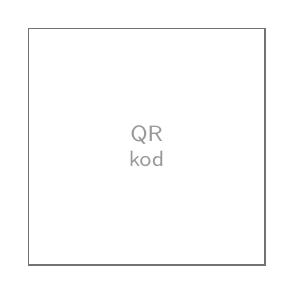
\begin{tikzpicture}
\draw[black!55,line width=0.6pt] (0,0) rectangle (30mm,30mm);
\node[black!40,font=\sffamily\fontsize{8}{9}\selectfont,align=center] at (15mm,15mm) {QR\\kod};
\end{tikzpicture}\\[1.5mm]
{\sffamily\fontsize{9}{11}\selectfont\color{black!70} #1}%
}

\arrayrulecolor{accent}
\setlength{\arrayrulewidth}{0.7pt}
\renewcommand{\arraystretch}{1.35}
\newcommand{\anstitle}[1]{{\sffamily\bfseries\color{accent}\fontsize{11}{13}\selectfont #1}\\[1.3mm]}

% ---- Shared reference diagram for Set 3: two parallel lines cut by a transversal,
% point P on l1, point Q on l2, four angle positions marked at each. ----
\newcommand{\transversaldiagram}{%
\begin{center}
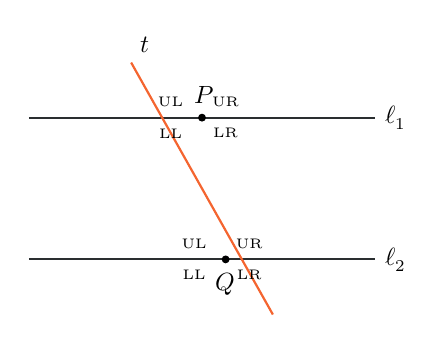
\begin{tikzpicture}[scale=1]
\draw[ink,thick] (-22mm,9mm) -- (22mm,9mm);
\node[right] at (22mm,9mm) {\small $\ell_1$};
\draw[ink,thick] (-22mm,-9mm) -- (22mm,-9mm);
\node[right] at (22mm,-9mm) {\small $\ell_2$};
\draw[accent,thick] (-9mm,16mm) -- (9mm,-16mm);
\node[above right] at (-9mm,16mm) {\small $t$};
\fill (0,9mm) circle (0.5mm);
\node[above] at (0,9.5mm) {\small $P$};
\fill (3mm,-9mm) circle (0.5mm);
\node[below] at (3mm,-9.5mm) {\small $Q$};
\node[font=\tiny] at (-4mm,11mm) {UL};
\node[font=\tiny] at (3mm,11mm) {UR};
\node[font=\tiny] at (-4mm,7mm) {LL};
\node[font=\tiny] at (3mm,7mm) {LR};
\node[font=\tiny] at (-1mm,-7mm) {UL};
\node[font=\tiny] at (6mm,-7mm) {UR};
\node[font=\tiny] at (-1mm,-11mm) {LL};
\node[font=\tiny] at (6mm,-11mm) {LR};
\end{tikzpicture}
\end{center}
}

\begin{document}

% ================= PAGE 1: Set 1 | Set 2 =================
\topicheader{19}{Burchaklar va Uchburchaklar}
\pagefooter{1}
\colrule{32}{238}
\mbox{}%

\begin{textblock*}{\COLW}(\LCOL,32mm)
{\fontsize{11.5}{14.5}\selectfont
\setkicker{1-to'plam}{To'ldiruvchi, yondosh va vertikal burchaklar.}

\noindent\pnum{1} Two angles are complementary. One measures $37°$. Find the other.\\[18mm]
\noindent\pnum{2} Two angles are supplementary. One measures $112°$. Find the other.\\[18mm]
\noindent\pnum{3} Two angles are vertical angles. One measures $74°$. Find the other.\\[18mm]
\noindent\pnum{4} Two complementary angles measure $2x$ and $3x$. Find $x$, then find both angles.\\[20mm]
\noindent\pnum{5} Two supplementary angles measure $4x+10$ and $2x+20$. Find $x$, then find both angles.\\[20mm]
\noindent\pnum{6} Two vertical angles measure $3x+15$ and $5x-25$. Find $x$, then find the angle.
}
\end{textblock*}

\begin{textblock*}{\COLW}(\RCOL,32mm)
{\fontsize{11.5}{14.5}\selectfont
\setkicker{2-to'plam}{Uchburchak ichki burchaklari yig'indisi.}

\noindent\pnum{1} A triangle has angles $50°$ and $65°$. Find the third angle.\\[18mm]
\noindent\pnum{2} A triangle has angles $90°$ and $35°$. Find the third angle.\\[18mm]
\noindent\pnum{3} An equilateral triangle has three equal angles, each $x$. Find $x$.\\[18mm]
\noindent\pnum{4} A triangle's angles measure $2x$, $3x$, and $4x$. Find $x$, then find each angle.\\[20mm]
\noindent\pnum{5} A triangle's angles measure $x+10$, $x+20$, and $x+30$. Find $x$, then find each angle.\\[20mm]
\noindent\pnum{6} An isosceles triangle has two equal base angles, each $2x$, and a vertex angle of $x+60$. Find $x$, then find all three angles.
}
\end{textblock*}

\clearpage

% ================= PAGE 2: Set 3 (diagram) | Set 4 =================
\topicheader{19}{Burchaklar va Uchburchaklar}
\pagefooter{2}
\colrule{32}{238}
\mbox{}%

\begin{textblock*}{\COLW}(\LCOL,32mm)
{\fontsize{11}{14}\selectfont
\setkicker{3-to'plam}{Parallel to'g'ri chiziqlar va kesuvchi. $\ell_1\parallel\ell_2$, kesuvchi $t$ ularni $P$ va $Q$ nuqtalarda kesadi.}
\transversaldiagram

\noindent\pnum{1} $P$'s lower-right angle is $72°$. Find $Q$'s upper-left angle.\\[10mm]
\noindent\pnum{2} $P$'s lower-left angle is $96°$. Find $Q$'s upper-right angle.\\[10mm]
\noindent\pnum{3} $P$'s lower-right angle is $130°$. Find $Q$'s upper-right angle.\\[10mm]
\noindent\pnum{4} $P$'s upper-right angle is $108°$. Find $Q$'s upper-right angle.\\[10mm]
\noindent\pnum{5} $P$'s lower-left angle is $85°$. Find $Q$'s lower-left angle.\\[10mm]
\noindent\pnum{6} Lines $m$ and $n$ cut by a transversal, $m\parallel n$ is \emph{not} stated. One angle is $85°$, the alternate-interior angle is $95°$. Can you conclude $m\parallel n$?
}
\end{textblock*}

\begin{textblock*}{\COLW}(\RCOL,32mm)
{\fontsize{10.5}{13.5}\selectfont
\setkicker{4-to'plam}{O'xshash uchburchaklar: harflar tartibiga rioya qiling.}

\noindent\pnum{1} $\triangle ABC \sim \triangle DEF$. $AB=4$, $BC=6$, $AC=8$, $DE=6$. Find $EF$ and $DF$.\\[14mm]
\noindent\pnum{2} $\triangle PQR \sim \triangle LMN$. $PQ=5$, $QR=12$, $PR=13$, $LM=15$. Find $MN$ and $LN$.\\[14mm]
\noindent\pnum{3} $\triangle XYZ \sim \triangle ABC$. $XY=7$, $YZ=9$, $XZ=11$, $BC=18$. Find $AB$ and $AC$.\\[14mm]
\noindent\pnum{4} $\triangle GHI \sim \triangle KLM$. $GH=10$, $HI=14$, $GI=16$, $KL=25$. Find $LM$ and $KM$.\\[14mm]
\noindent\pnum{5} $\triangle RST \sim \triangle UVW$, scale $\frac{3}{2}$ (RST$\to$UVW). $RS=8$, $ST=10$, $RT=14$. Find $UV,VW,UW$.\\[14mm]
\noindent\pnum{6} $\triangle ABC \sim \triangle DEF$. $AB=6$, $BC=8$, $AC=10$ (perimeter $24$), $DE=9$. Find the perimeter of $\triangle DEF$.
}
\end{textblock*}

\clearpage

% ================= PAGE 3: Set 5 | Set 6 (spot the error) =================
\topicheader{19}{Burchaklar va Uchburchaklar}
\pagefooter{3}
\colrule{32}{238}
\mbox{}%

\begin{textblock*}{\COLW}(\LCOL,32mm)
{\fontsize{10.3}{13}\selectfont
\setkicker{5-to'plam}{Aralash: burchaklar + o'xshashlik.}

\noindent\pnum{1} In $\triangle ABC$, $\angle A=50°$, $\angle B=70°$. Find $\angle C$. Also $\triangle ABC \sim \triangle DEF$, $DE=2\times AB$; if $AB=6$, find $DE$ and state $\angle D$ (explain why, no new computation).\\[12mm]
\noindent\pnum{2} Two triangles have $\angle A=\angle D=65°$, $\angle B=\angle E=80°$. Are they similar? By which criterion? Find $\angle C,\angle F$.\\[10mm]
\noindent\pnum{3} $\triangle ABC \sim \triangle DEF$ by SAS: $AB=8$, $DE=12$, $\angle A=\angle D=40°$, $AC=10$. Find $DF$.\\[10mm]
\noindent\pnum{4} In $\triangle ABC$, $D$ on $AB$, $E$ on $AC$, $DE\parallel BC$. $AD=4$, $DB=6$, $AE=6$. Find $EC$.\\[10mm]
\noindent\pnum{5} A $1.8$ m person casts a $2.4$ m shadow. A flagpole casts a $9.6$ m shadow. Find the flagpole's height.\\[10mm]
\noindent\pnum{6} Two triangles both have angles $55°,60°,65°$. First triangle's side opposite $55°$ is $5$; second's is $10$. Are they similar? Find the scale factor.
}
\end{textblock*}

\begin{textblock*}{\COLW}(\RCOL,32mm)
{\fontsize{10}{13}\selectfont
\setkicker{6-to'plam}{Xatoni toping -- buzilgan qadamni ayting, to'g'ri javobni bering.}

\noindent\pnum{1} $\ell_1\parallel\ell_2$. $P$'s lower-right angle is $70°$. Find $Q$'s upper-left angle.\\[1mm]
\hspace*{7mm}\textit{``Bular bir tomonlama ichki burchaklar: $180-70=110°$.''}\\[2mm]
\hspace*{7mm}Xato va to'g'ri javob: \makebox[52mm]{\dotfill}\\[6mm]

\noindent\pnum{2} Uchburchak burchaklari $2x,3x,4x$. $x$ ni toping.\\[1mm]
\hspace*{7mm}\textit{``$2x+3x+4x=360$, $9x=360$, $x=40$.''}\\[2mm]
\hspace*{7mm}Xato va to'g'ri javob: \makebox[52mm]{\dotfill}\\[6mm]

\noindent\pnum{3} $\triangle ABC\sim\triangle DEF$. $AB=6,BC=9,AC=12,DE=8$. $EF$ ni toping.\\[1mm]
\hspace*{7mm}\textit{``$EF=AC\times\frac{DE}{AB}=12\times\frac86=16$.''}\\[2mm]
\hspace*{7mm}Xato va to'g'ri javob: \makebox[52mm]{\dotfill}\\[6mm]

\noindent\pnum{4} Ikki burchak komplementar. Biri $65°$. Ikkinchisini toping.\\[1mm]
\hspace*{7mm}\textit{``Yig'indi $180°$: $180-65=115°$.''}\\[2mm]
\hspace*{7mm}Xato va to'g'ri javob: \makebox[52mm]{\dotfill}\\[6mm]

\noindent\pnum{5} $\ell_1\parallel\ell_2$. $P$'s upper-right (mos burchak) $112°$. $Q$'s upper-right?\\[1mm]
\hspace*{7mm}\textit{``Mos burchaklar yig'indisi $180°$: $180-112=68°$.''}\\[2mm]
\hspace*{7mm}Xato va to'g'ri javob: \makebox[52mm]{\dotfill}
}
\end{textblock*}

\clearpage

% ================= PAGE 4: Set 7 (bonus) =================
\topicheader{19}{Burchaklar va Uchburchaklar}
\pagefooter{4}
\colrule{32}{238}
\mbox{}%

\begin{textblock*}{\COLW}(\LCOL,32mm)
{\fontsize{10.8}{14}\selectfont
\setkicker{7-to'plam}{Bonus / qiyin -- ko'p qadamli masalalar.}

\noindent\pnum{1} In $\triangle ABC$, $\angle A=3x$, $\angle B=2x+10$, $\angle C=x+20$. Find $x$ and all three angles, then classify as acute, right, or obtuse.\\[24mm]
\noindent\pnum{2} $\ell_1\parallel\ell_2$. $P$'s lower-left angle is $4y+10$. $Q$'s upper-left is $6y-50$ (co-interior pair). Find $y$, then both angles.\\[24mm]
\noindent\pnum{3} $\triangle ABC \sim \triangle DEF$. Perimeter of $ABC$ is $30$, $AB:BC:AC=2:3:5$. $DE=10$. Find the perimeter of $DEF$ (and $EF$, $DF$).\\[24mm]
\noindent\pnum{4} An isosceles triangle has vertex angle $3x-10$ and each base angle $x+15$. Find $x$, all three angles, and the exterior angle at a base angle.\\[24mm]
\noindent\pnum{5} A $3$ m stick casts a $4$ m shadow. A tree casts a $16$ m shadow. (a) Find the tree's height. (b) Find the straight-line distance from the top of the tree to the tip of its shadow.
}
\end{textblock*}

\clearpage

% ================= PAGE 5: Javoblar =================
\topicheader{19}{Burchaklar va Uchburchaklar}
\pagefooter{5}
\mbox{}%

\begin{textblock*}{194mm}(16mm,30mm)
{\bfseries\itshape\color{accent}\fontsize{19}{21}\selectfont\centering Javoblar\par}
\end{textblock*}

\begin{textblock*}{194mm}(16mm,44mm)
{\fontsize{8.7}{11}\selectfont
\centering
\renewcommand{\arraystretch}{1.3}
\begin{tabular}{|>{\centering\arraybackslash}p{24mm}|>{\centering\arraybackslash}p{8mm}|>{\centering\arraybackslash}p{44mm}|>{\centering\arraybackslash}p{8mm}|>{\centering\arraybackslash}p{44mm}|}
\hline
\rowcolor{badge!55}\textbf{To'plam} & \textbf{\#} & \textbf{Javob} & \textbf{\#} & \textbf{Javob}\\
\hline
\multirow{3}{24mm}{\centering 1-to'plam} & 1 & $53°$ & 2 & $68°$\\\cline{2-5}
 & 3 & $74°$ & 4 & $x=18$; $36°,54°$\\\cline{2-5}
 & 5 & $x=25$; $110°,70°$ & 6 & $x=20$; $75°$\\\hline
\multirow{3}{24mm}{\centering 2-to'plam} & 1 & $65°$ & 2 & $55°$\\\cline{2-5}
 & 3 & $x=60°$ & 4 & $x=20$; $40°,60°,80°$\\\cline{2-5}
 & 5 & $x=40$; $50°,60°,70°$ & 6 & $x=24$; $48°,48°,84°$\\\hline
\multirow{3}{24mm}{\centering 3-to'plam} & 1 & $72°$ (almashinuvchi) & 2 & $96°$ (almashinuvchi)\\\cline{2-5}
 & 3 & $50°$ (bir tomonlama) & 4 & $108°$ (mos burchak)\\\cline{2-5}
 & 5 & $85°$ (mos burchak) & 6 & Yo'q, $m\not\parallel n$\\\hline
\multirow{3}{24mm}{\centering 4-to'plam} & 1 & $\frac32$; $EF=9,DF=12$ & 2 & $3$; $MN=36,LN=39$\\\cline{2-5}
 & 3 & $2$; $AB=14,AC=22$ & 4 & $\frac52$; $LM=35,KM=40$\\\cline{2-5}
 & 5 & $UV=12,VW=15,UW=21$ & 6 & $\frac32$; perimetr $36$\\\hline
\multirow{3}{24mm}{\centering 5-to'plam} & 1 & $60°$; $DE=12,\angle D=50°$ & 2 & Ha, AA; $35°,35°$\\\cline{2-5}
 & 3 & $DF=15$ & 4 & $EC=9$\\\cline{2-5}
 & 5 & $7.2$ m & 6 & Ha, AA; koeffitsiyent $2$\\\hline
\multirow{5}{24mm}{\centering 6-to'plam} & \multicolumn{4}{p{104mm}|}{1.\ Xato -- bular almashinuvchi ichki (teng), bir tomonlama emas. To'g'ri: $70°$.}\\\cline{2-5}
 & \multicolumn{4}{p{104mm}|}{2.\ Xato -- uchburchak burchaklari yig'indisi $180°$, $360°$ emas. To'g'ri: $x=20$.}\\\cline{2-5}
 & \multicolumn{4}{p{104mm}|}{3.\ Xato -- mos tomon $BC$, $AC$ emas. To'g'ri: $EF=9\times\frac86=12$.}\\\cline{2-5}
 & \multicolumn{4}{p{104mm}|}{4.\ Xato -- komplementar yig'indisi $90°$. To'g'ri: $25°$.}\\\cline{2-5}
 & \multicolumn{4}{p{104mm}|}{5.\ Xato -- mos burchaklar teng, yig'indi emas. To'g'ri: $112°$.}\\\hline
\multirow{5}{24mm}{\centering 7-to'plam} & \multicolumn{4}{p{104mm}|}{1.\ $x=25$; $75°,60°,45°$ -- o'tkir uchburchak.}\\\cline{2-5}
 & \multicolumn{4}{p{104mm}|}{2.\ $y=22$; $P=98°,Q=82°$.}\\\cline{2-5}
 & \multicolumn{4}{p{104mm}|}{3.\ $AB{=}6,BC{=}9,AC{=}15$; koeff.\ $\frac53$; $EF{=}15,DF{=}25$; perimetr $50$.}\\\cline{2-5}
 & \multicolumn{4}{p{104mm}|}{4.\ $x=32$; uch $86°$, asos $47°,47°$; tashqi burchak $133°$.}\\\cline{2-5}
 & \multicolumn{4}{p{104mm}|}{5.\ (a) balandlik $12$ m (b) masofa $=\sqrt{12^2+16^2}=20$ m.}\\\hline
\end{tabular}
}
\end{textblock*}

\begin{textblock*}{194mm}(16mm,252mm)
\centering
{\sffamily\fontsize{9.5}{11.5}\selectfont\color{black!70} Video yechimlar va qo'shimcha testlar uchun quyidagi QR kodlarni skanerlang:}\\[4mm]
\begin{minipage}[t]{32mm}\centering\qrbox{YouTube}\end{minipage}%
\hspace{16mm}%
\begin{minipage}[t]{32mm}\centering\qrbox{Telegram}\end{minipage}
\end{textblock*}

\end{document}
